\normaltrue \difficilefalse \tdifficilefalse
\correctionfalse

%\UPSTIidClasse{11} % 11 sup, 12 spé
%\newcommand{\UPSTIidClasse}{11}

\exer{Boitier différentiel$\star$ \label{G2:01:2001}}
\setcounter{question}{0}\UPSTIcompetence[2]{G2-01}
\index{Compétence G2-01}

\ifcorrection
\else
\textbf{Pas de corrigé pour cet exercice.}
\fi


\ifprof 
\else
Soit la pièce suivante.
\begin{center}
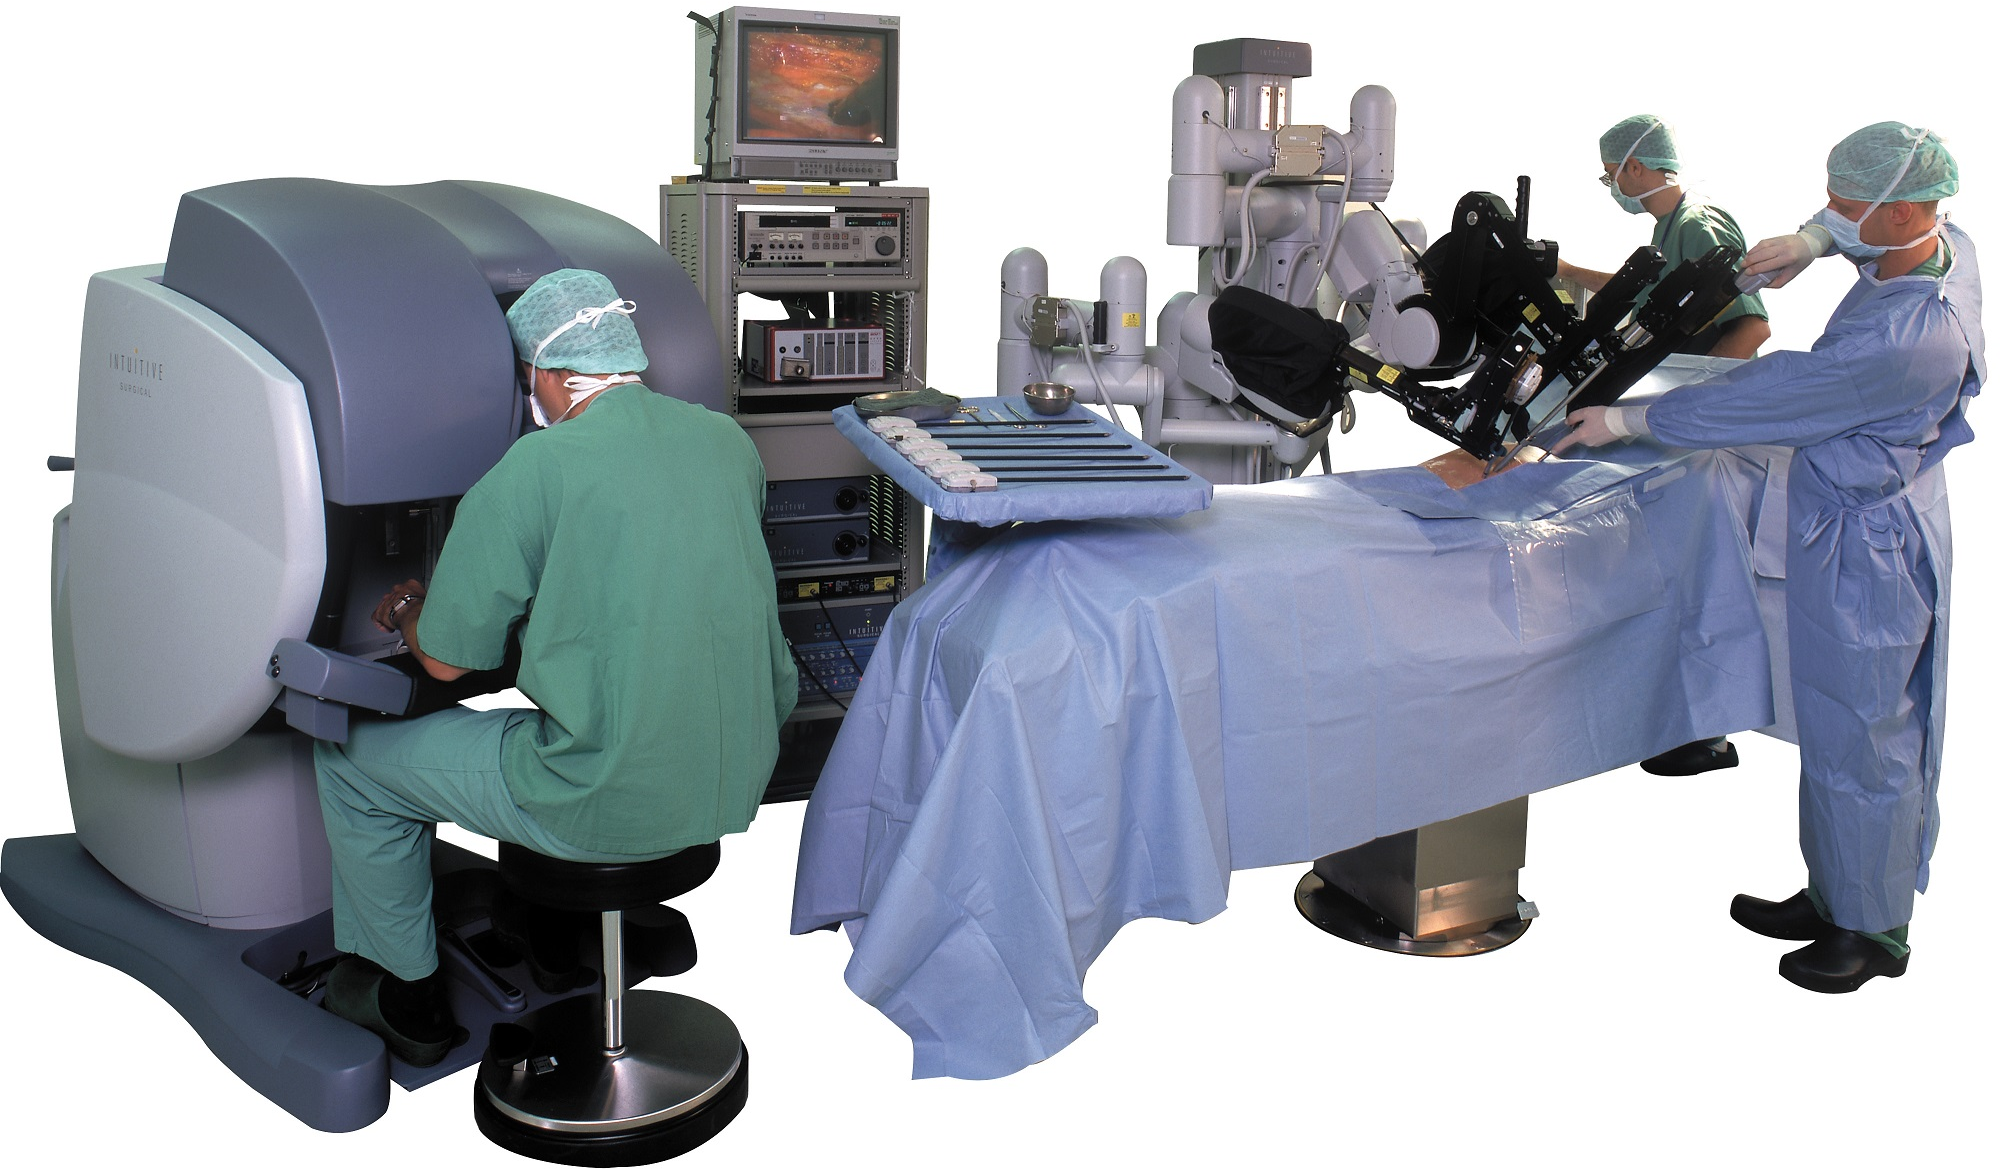
\includegraphics[width=.9\linewidth]{fig_01}
\end{center}
 \fi
 
\question{Proposer une gamme de fabrication, de l'élaboration du brut à la finition.}
\ifprof
\begin{center}
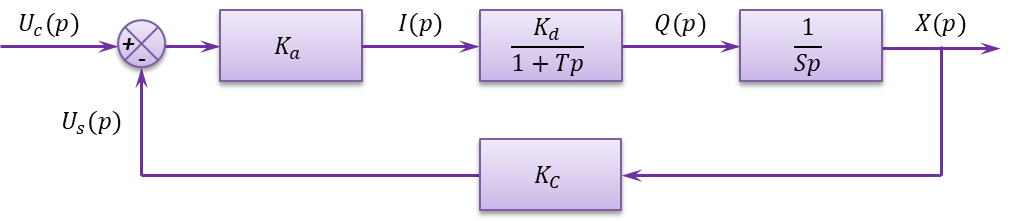
\includegraphics[width=.9\linewidth]{cor_01}
\end{center}

\else 
\fi

Le dessin de défintion précise les notes suivantes. 
\begin{center}
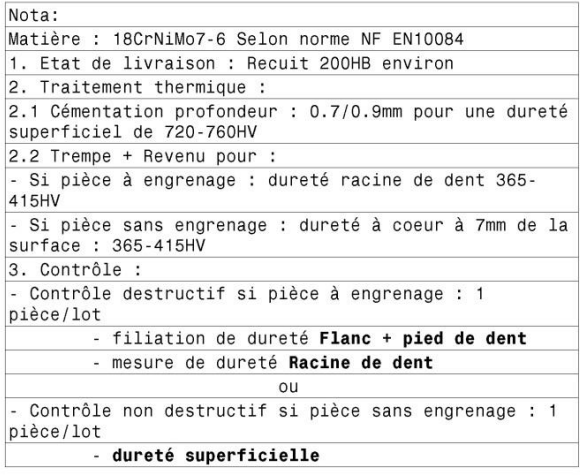
\includegraphics[width=.9\linewidth]{fig_02}
\end{center}

\question{18CrNiMo7-6 désigne l'acier avec lequel est construit la pièce. Qu'est-ce qu'un acier ?}

\question{Avant usinage la pièce est livrée avec un état Recuit 200HB. Que signifie 200 HB ? Détailler l'essai permettant d'obtenir cette valeur.}

\question{La dureté à coeur à 7mm de la surface doit être comprise entre 365 et 415 HV ? Que signifie cette indication ? Détailler l'essai permettant d'obtenir cette valeur.}

\ifprof
\else
\begin{flushright}
\footnotesize{Corrigé  voir \ref{G2:01:2001}.}
\end{flushright}%
\fi